%---------------------- % % % Personnalisation des couleurs % % % ---------- MARRON-ROUGE -------
\definecolor{couleurFonce}{RGB}{103,45,50} % Couleur du Code APOGEE
\definecolor{couleurClaire}{RGB}{210,135,160} % Couleur du fond de la bande
\definecolor{couleurTexte}{RGB}{255,255,255} % Couleur du texte de la bande
%------------------------------------------------------------------------------------------


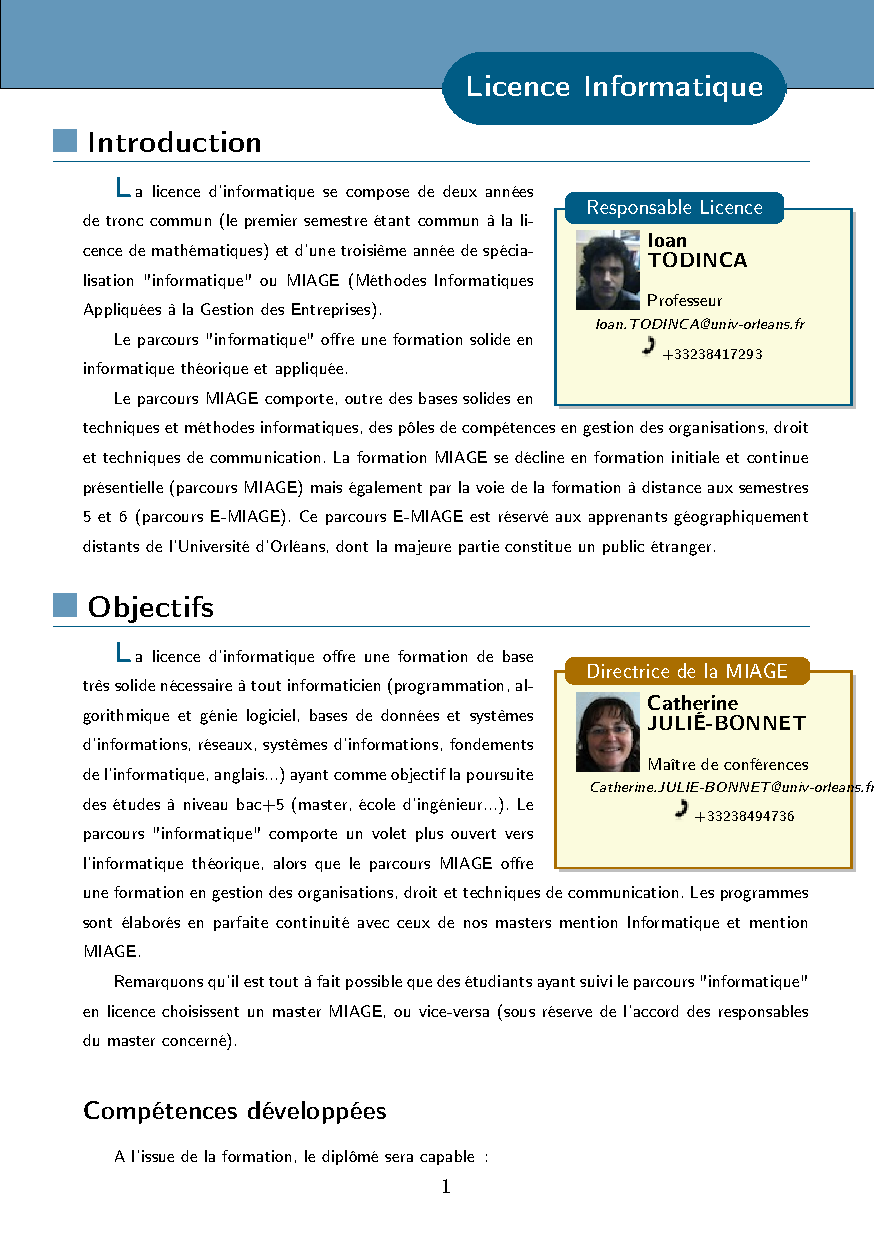
\includepdf[fitpaper,pages=-]{Preambule_Info_MasterMoCaHP_S1S2.pdf}

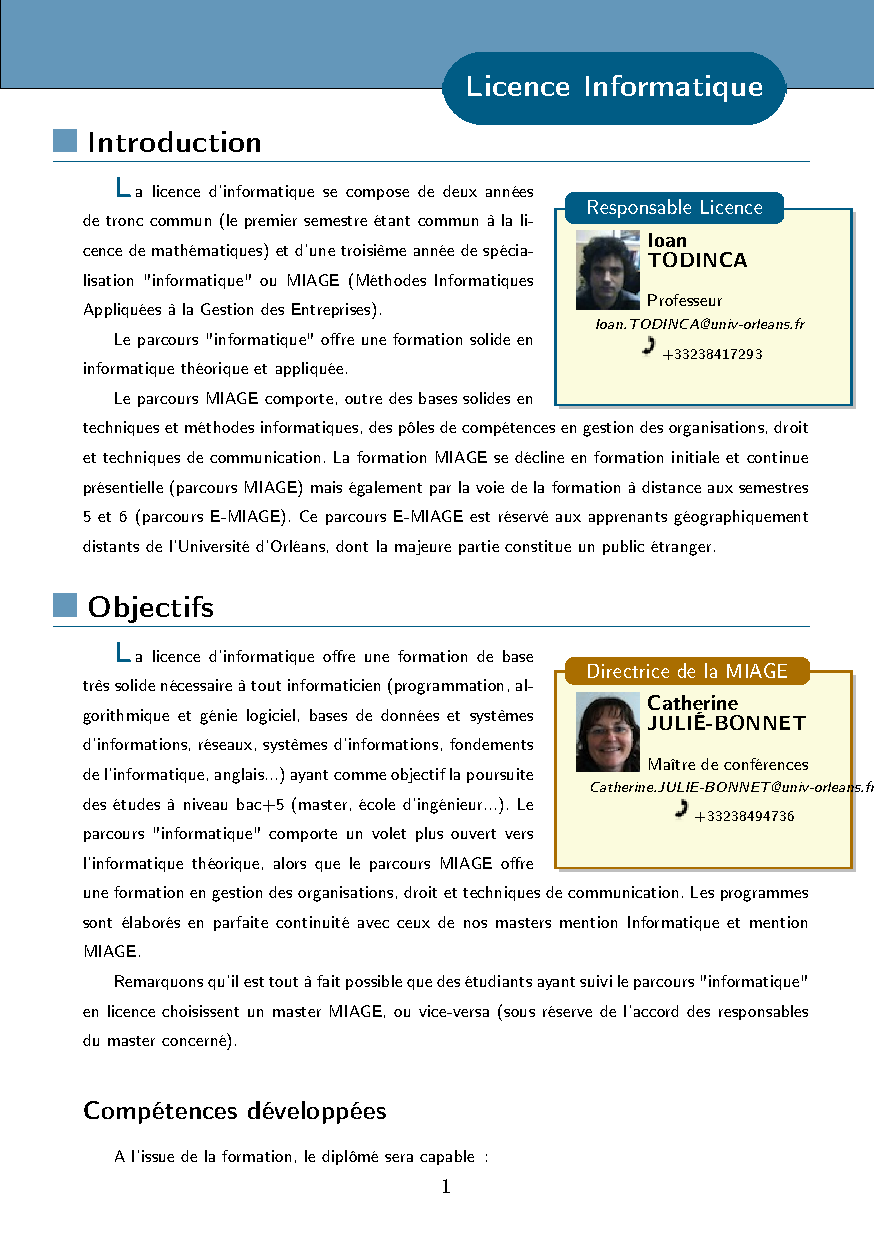
\includepdf[fitpaper,pages=-]{Preambule_Info_MasterMoCaHP_S3S4.pdf}

%==========================================================================================
% SEMESTRE 1
%==========================================================================================
\module[codeApogee={UE 11}, 
titre={Mise à niveau en informatique}, 
CODEUE={1}, 
COURS={10}, 
TD={}, 
TP={15}, 
CTD={}, 
TOTAL={25}, 
SEMESTRE={Semestre 1}, 
COEFF={1}, 
ECTS={1}, 
MethodeEval={Contrôle continue et terminal}, 
ModalitesCCSemestreUn={CC et CT}, 
ModalitesCCSemestreDeux={CT}, 
%CalculNFSessionUne={$\frac{(CC+2*CT)}{3}$}, 
%CalculNFSessionDeux={CT}, 
NoteEliminatoire={7}, 
nomPremierResp={Prénom NOM}, 
emailPremierResp={Prenom.NOM@univ-orleans.fr}, 
nomSecondResp={}, 
emailSecondResp={}, 
langue={Français}, 
nbPrerequis={1}, 
descriptionCourte={true}, 
descriptionLongue={true}, 
objectifs={true}, 
ressources={true}, 
bibliographie={false}] 
{
Unité obligatoire pour les titulaires d\'une licence de mathématiques.
} 
{
\begin{itemize} 
  \item programmation impérative en C : constructions de base du langage C
  \item programmation impérative en C : gestion de la mémoire
  \item programmation impérative en C : pratique avec gcc, make et gdb
  \item analyse des algorithmes : complexités asymptotiques, tris, strassen
  \item introduction à la programmation en C++ 
\end{itemize} 
} 
{Notions de programmation impérative et objet en Java} 
{\begin{itemize}
\ObjItem Savoir écrire des programmes C qui manipulent des pointeurs, en particulier pour utiliser MPI dans le module "Programmation parallèle".
\ObjItem Avoir les bases pour analyser la complexité d\'algorithmes séquentiels pour pouvoir dans le même module analyser des algorithmes parallèles.
\end{itemize}
} 
{Ressources} 
{Biblio} 
 
\vfill

%==========================================================================================
\module[codeApogee={UE 11}, 
titre={Mise à niveau en mathématique}, 
CODEUE={1}, 
COURS={10}, 
TD={15}, 
TP={}, 
CTD={}, 
TOTAL={25}, 
SEMESTRE={}, 
COEFF={1}, 
ECTS={1}, 
MethodeEval={Contrôle continue et terminal}, 
ModalitesCCSemestreUn={CC et CT}, 
ModalitesCCSemestreDeux={CT}, 
%CalculNFSessionUne={$\frac{(CC+2*CT)}{3}$}, 
%CalculNFSessionDeux={CT}, 
NoteEliminatoire={7}, 
nomPremierResp={Prénom NOM}, 
emailPremierResp={Prenom.NOM@univ-orleans.fr}, 
nomSecondResp={}, 
emailSecondResp={}, 
langue={Français}, 
nbPrerequis={0}, 
descriptionCourte={true}, 
descriptionLongue={true}, 
objectifs={true}, 
ressources={true}, 
bibliographie={false}] 
{
Unité obligatoire pour les titulaires d\'une licence d\'informatique.
} 
{
DESCRIPTION-CONTENU 
} 
{} 
{\begin{itemize}
\ObjItem Objectif 
\ObjItem Objectif
\end{itemize} 
} 
{Ressources} 
{Biblio} 
 
\vfill

%==========================================================================================
\module[codeApogee={UE 12}, 
titre={Système et réseaux}, 
CODEUE={1}, 
COURS={20}, 
TD={20}, 
TP={30}, 
CTD={}, 
TOTAL={70}, 
SEMESTRE={Semestre 1}, 
COEFF={6}, 
ECTS={6}, 
MethodeEval={Contrôle continue et terminal}, 
ModalitesCCSemestreUn={CC et CT}, 
ModalitesCCSemestreDeux={CT}, 
%CalculNFSessionUne={$\frac{(CC+2*CT)}{3}$}, 
%CalculNFSessionDeux={CT}, 
NoteEliminatoire={7}, 
nomPremierResp={Nicolas OLLINGER}, 
emailPremierResp={Nicolas.OLLINGER@univ-orleans.fr}, 
nomSecondResp={Sophie ROBERT}, 
emailSecondResp={Sophie.ROBERT@univ-orleans.fr}, 
langue={Français}, 
nbPrerequis={1}, 
descriptionCourte={true}, 
descriptionLongue={true}, 
objectifs={true}, 
ressources={true}, 
bibliographie={false}] 
{
Unité obligatoire pour les titulaires d\'une licence de mathématiques. 
} 
{
\begin{itemize} 
  \item Architecture de systèmes d\'exploitation
  \item Utilisation d\'Unix
  \item Administration Unix et windows
  \item Architecture des réseaux : structure en couches, protocoles, services
  \item Réseaux locaux sous UDP-TCP/IP, Ethernet
  \item Protocoles de routage : RIP, OSPF, BGP
  \item Principaux protocoles Internet : DNS (annuaire de noms de domaines) SMTP (mail), FTP (transfert de fichiers), HTTP (web) ... 
\end{itemize} 
} 
{Module de remise à niveau} 
{\begin{itemize}
\ObjItem Utilisation et administration de systèmes d\'exploitation 
\ObjItem Principes et pratique des réseaux locaux informatiques
\end{itemize} 
} 
{Ressources} 
{Biblio} 
 
\vfill

%==========================================================================================
\module[codeApogee={UE 12}, 
titre={Mathématiques}, 
CODEUE={1}, 
COURS={35}, 
TD={35}, 
TP={}, 
CTD={}, 
TOTAL={70}, 
SEMESTRE={}, 
COEFF={6}, 
ECTS={6}, 
MethodeEval={Contrôle continue et terminal}, 
ModalitesCCSemestreUn={CC et CT}, 
ModalitesCCSemestreDeux={CT}, 
%CalculNFSessionUne={$\frac{(CC+2*CT)}{3}$}, 
%CalculNFSessionDeux={CT}, 
NoteEliminatoire={7}, 
nomPremierResp={Prénom NOM}, 
emailPremierResp={Prenom.NOM@univ-orleans.fr}, 
nomSecondResp={}, 
emailSecondResp={}, 
langue={Français}, 
nbPrerequis={0}, 
descriptionCourte={true}, 
descriptionLongue={true}, 
objectifs={true}, 
ressources={true}, 
bibliographie={false}] 
{
Unité obligatoire pour les titulaires d\'une licence d\'informatique. 
} 
{
DESCRIPTION-CONTENU 
} 
{} 
{\begin{itemize}
\ObjItem Objectif 
\ObjItem Objectif
\end{itemize} 
} 
{Ressources} 
{Biblio} 
 
\vfill

%==========================================================================================
\module[codeApogee={UE 13}, 
titre={Anglais}, 
CODEUE={1}, 
COURS={}, 
TD={24}, 
TP={}, 
CTD={}, 
TOTAL={24}, 
SEMESTRE={}, 
COEFF={2}, 
ECTS={2}, 
MethodeEval={Contrôle continue et terminal}, 
ModalitesCCSemestreUn={CC et CT}, 
ModalitesCCSemestreDeux={CT}, 
%CalculNFSessionUne={$\frac{(CC+2*CT)}{3}$}, 
%CalculNFSessionDeux={CT}, 
NoteEliminatoire={7}, 
nomPremierResp={Prénom NOM}, 
emailPremierResp={Prenom.NOM@univ-orleans.fr}, 
nomSecondResp={}, 
emailSecondResp={}, 
langue={Français}, 
nbPrerequis={0}, 
descriptionCourte={true}, 
descriptionLongue={true}, 
objectifs={true}, 
ressources={true}, 
bibliographie={false}] 
{
Unité obligatoire. 
} 
{
DESCRIPTION-CONTENU 
} 
{} 
{\begin{itemize}
\ObjItem Objectif 
\ObjItem Objectif
\end{itemize} 
} 
{Ressources} 
{Biblio} 
 
\vfill

%==========================================================================================
\module[codeApogee={UE 14}, 
titre={Signal, filtrage, EDP (Théorie et pratique)}, 
CODEUE={1}, 
COURS={30}, 
TD={30}, 
TP={}, 
CTD={}, 
TOTAL={60}, 
SEMESTRE={}, 
COEFF={7}, 
ECTS={7}, 
MethodeEval={Contrôle continue et terminal}, 
ModalitesCCSemestreUn={CC et CT}, 
ModalitesCCSemestreDeux={CT}, 
%CalculNFSessionUne={$\frac{(CC+2*CT)}{3}$}, 
%CalculNFSessionDeux={CT}, 
NoteEliminatoire={7}, 
nomPremierResp={Prénom NOM}, 
emailPremierResp={Prenom.NOM@univ-orleans.fr}, 
nomSecondResp={}, 
emailSecondResp={}, 
langue={Français}, 
nbPrerequis={0}, 
descriptionCourte={true}, 
descriptionLongue={true}, 
objectifs={true}, 
ressources={true}, 
bibliographie={false}] 
{
Unité obligatoire. 
} 
{
\begin{itemize} 
  \item Filtres-systèmes.
  \item Analyse spectrale des signaux analogiques.
  \item Analyse spectrale des signaux numériques ( TFD, FFT).
  \item Spectrogramme.
  \item Echantillonnage - Théorème de Shannon - Analyse temps-fréquence.
  \item Transformation  de Laplace - Transformée en z.
  \item Filtres idéaux -réels - Fonctions de transfert - Filtres différentiels.
  \item Filtres à réponse impulsionnelle finie  (RIF).
  \item Application au signal sonore.
  \item Méthodes des EDP.
  \item Mise en \oe uvre numérique (Scilab). 
\end{itemize} 
} 
{} 
{\begin{itemize}
\ObjItem Objectif 
\ObjItem Objectif
\end{itemize} 
} 
{Ressources} 
{Biblio} 
 
\vfill

%==========================================================================================
\module[codeApogee={UE 15}, 
titre={Génie logiciel pour le calcul haute performance}, 
CODEUE={1}, 
COURS={16}, 
TD={20}, 
TP={}, 
CTD={}, 
TOTAL={36}, 
SEMESTRE={}, 
COEFF={4}, 
ECTS={4}, 
MethodeEval={Contrôle continue et terminal}, 
ModalitesCCSemestreUn={CC et CT}, 
ModalitesCCSemestreDeux={CT}, 
%CalculNFSessionUne={$\frac{(CC+2*CT)}{3}$}, 
%CalculNFSessionDeux={CT}, 
NoteEliminatoire={7}, 
nomPremierResp={Prénom NOM}, 
emailPremierResp={Prenom.NOM@univ-orleans.fr}, 
nomSecondResp={}, 
emailSecondResp={}, 
langue={Français}, 
nbPrerequis={1}, 
descriptionCourte={true}, 
descriptionLongue={true}, 
objectifs={true}, 
ressources={true}, 
bibliographie={false}] 
{
Unité obligatoire.
} 
{
\begin{itemize} 
  \item  Introduction au génie logiciel
  \item  Tests unitaires, de programmes séquentiels, de programmes parallèles
  \item  Débogage de programmes séquentiels, parallèles
  \item  Profilage pour les performances de programmes séquentiels, parallèles 
\end{itemize} 
} 
{Programmation impérative}
{\begin{itemize}
\ObjItem A l\'issue de cette UE les étudiants devront être capables de participer à un développement logiciel rigoureux dans le cadre spécifique d\'applications de calcul haute performance. 

\end{itemize} 
} 
{Ressources} 
{Biblio} 
 
\vfill

%==========================================================================================
\module[codeApogee={UE 16}, 
titre={Modélisation, graphes et algorithmes}, 
CODEUE={1}, 
COURS={16}, 
TD={20}, 
TP={}, 
CTD={}, 
TOTAL={36}, 
SEMESTRE={}, 
COEFF={4}, 
ECTS={4}, 
MethodeEval={Contrôle continue et terminal}, 
ModalitesCCSemestreUn={CC et CT}, 
ModalitesCCSemestreDeux={CT}, 
%CalculNFSessionUne={$\frac{(CC+2*CT)}{3}$}, 
%CalculNFSessionDeux={CT}, 
NoteEliminatoire={7}, 
nomPremierResp={Prénom NOM}, 
emailPremierResp={Prenom.NOM@univ-orleans.fr}, 
nomSecondResp={}, 
emailSecondResp={}, 
langue={Français}, 
nbPrerequis={0}, 
descriptionCourte={true}, 
descriptionLongue={true}, 
objectifs={true}, 
ressources={true}, 
bibliographie={false}] 
{
Unité obligatoire.
} 
{
DESCRIPTION-CONTENU 
} 
{} 
{\begin{itemize}
\ObjItem Objectif 
\ObjItem Objectif
\end{itemize} 
} 
{Ressources} 
{Biblio} 
 
\vfill

%==========================================================================================
\module[codeApogee={UE 17}, 
titre={Programmation parallèle}, 
CODEUE={1}, 
COURS={16}, 
TD={20}, 
TP={}, 
CTD={}, 
TOTAL={36}, 
SEMESTRE={}, 
COEFF={4}, 
ECTS={4}, 
MethodeEval={Contrôle continue et terminal}, 
ModalitesCCSemestreUn={CC et CT}, 
ModalitesCCSemestreDeux={CT}, 
%CalculNFSessionUne={$\frac{(CC+2*CT)}{3}$}, 
%CalculNFSessionDeux={CT}, 
NoteEliminatoire={7}, 
nomPremierResp={Prénom NOM}, 
emailPremierResp={Prenom.NOM@univ-orleans.fr}, 
nomSecondResp={}, 
emailSecondResp={}, 
langue={Français}, 
nbPrerequis={0}, 
descriptionCourte={true}, 
descriptionLongue={true}, 
objectifs={true}, 
ressources={true}, 
bibliographie={false}] 
{
Unité obligatoire.
} 
{
DESCRIPTION-CONTENU 
} 
{} 
{\begin{itemize}
\ObjItem Objectif 
\ObjItem Objectif
\end{itemize} 
} 
{Ressources} 
{Biblio} 
 
\vfill

%==========================================================================================
\module[codeApogee={UE 18}, 
titre={Langages de scripts}, 
CODEUE={1}, 
COURS={10}, 
TD={10}, 
TP={}, 
CTD={}, 
TOTAL={20}, 
SEMESTRE={}, 
COEFF={2}, 
ECTS={2}, 
MethodeEval={Contrôle continue et terminal}, 
ModalitesCCSemestreUn={CC et CT}, 
ModalitesCCSemestreDeux={CT}, 
%CalculNFSessionUne={$\frac{(CC+2*CT)}{3}$}, 
%CalculNFSessionDeux={CT}, 
NoteEliminatoire={7}, 
nomPremierResp={Prénom NOM}, 
emailPremierResp={Prenom.NOM@univ-orleans.fr}, 
nomSecondResp={}, 
emailSecondResp={}, 
langue={Français}, 
nbPrerequis={1}, 
descriptionCourte={true}, 
descriptionLongue={true}, 
objectifs={true}, 
ressources={true}, 
bibliographie={false}] 
{
Unité obligatoire.
} 
{
Les applications de calcul scientifique et de simulations font très souvent appel à des bibliothèques ou même des applications complètes qui sont réutilisées. Dans ce contexte l\'interfaçage pour manier plusieurs bibliothèques ou applications peut s\'écrire à l\'aide de langages de scripts. Certains langages peuvent même être utilisés comme langages de prototypage rapide d\'applications de calcul haute performance, ou comme langage de développement rapide avec des performances acceptables pour des programmes ne devant s\'exécuter qu\'une seule fois ou peu de fois. Cette UE présentera un tel langage de scripts et pour ces utilisations. 
} 
{Programmation impérative et objet} 
{\begin{itemize}
\ObjItem A l\'issue de cette UE les étudiants devront être capables de prendre en main rapidement de nouveaux langages de scripts et devront être opérationnels dans l\'utilisation du langage présenté dans l\'UE pour le prototypage d\'applications de calcul haute performance. 

\end{itemize} 
} 
{Ressources} 
{Biblio} 
 
\vfill

%==========================================================================================
\module[codeApogee={UE 21}, 
titre={Algorithmique répartie}, 
CODEUE={1}, 
COURS={16}, 
TD={20}, 
TP={}, 
CTD={}, 
TOTAL={36}, 
SEMESTRE={}, 
COEFF={4}, 
ECTS={4}, 
MethodeEval={Contrôle continue et terminal}, 
ModalitesCCSemestreUn={CC et CT}, 
ModalitesCCSemestreDeux={CT}, 
%CalculNFSessionUne={$\frac{(CC+2*CT)}{3}$}, 
%CalculNFSessionDeux={CT}, 
NoteEliminatoire={7}, 
nomPremierResp={Prénom NOM}, 
emailPremierResp={Prenom.NOM@univ-orleans.fr}, 
nomSecondResp={}, 
emailSecondResp={}, 
langue={Français}, 
nbPrerequis={0}, 
descriptionCourte={true}, 
descriptionLongue={true}, 
objectifs={true}, 
ressources={true}, 
bibliographie={false}] 
{
Unité obligatoire.
} 
{
DESCRIPTION-CONTENU 
} 
{} 
{\begin{itemize}
\ObjItem Objectif 
\ObjItem Objectif
\end{itemize} 
} 
{Ressources} 
{Biblio} 
 
\vfill

%==========================================================================================
\module[codeApogee={UE 22}, 
titre={Analyse de données et méthodes de simulation}, 
CODEUE={1}, 
COURS={30}, 
TD={30}, 
TP={}, 
CTD={}, 
TOTAL={60}, 
SEMESTRE={}, 
COEFF={5}, 
ECTS={5}, 
MethodeEval={Contrôle continue et terminal}, 
ModalitesCCSemestreUn={CC et CT}, 
ModalitesCCSemestreDeux={CT}, 
%CalculNFSessionUne={$\frac{(CC+2*CT)}{3}$}, 
%CalculNFSessionDeux={CT}, 
NoteEliminatoire={7}, 
nomPremierResp={Prénom NOM}, 
emailPremierResp={Prenom.NOM@univ-orleans.fr}, 
nomSecondResp={}, 
emailSecondResp={}, 
langue={Français}, 
nbPrerequis={0}, 
descriptionCourte={true}, 
descriptionLongue={true}, 
objectifs={true}, 
ressources={true}, 
bibliographie={false}] 
{
Unité obligatoire.
} 
{
\begin{itemize} 
  \item Rappels sur l\'Analyse en Composantes Principales (ACP); Analyse Factorielle des Correspondances (AFC). Analyse des Correspondances Multiples (ACM), méthodes de Classification (hiérarchique et non hiérarchique), Analyse Discriminante. Applications à des jeux de données exemples (sous SAS et R).
  \item Méthodes de simulation: Simulation de variables aléatoires iid; méthodes d\'inversion, acceptation-rejet, polaire. 
  \item Méthodes de Monte-Carlo; usage de la Loi des grands Nombres et du Théorème de Limite Centrale;  calcul d\'intégrales, réduction de variance; simulation de systèmes complexes. 
\end{itemize} 
} 
{} 
{\begin{itemize}
\ObjItem Objectif 
\ObjItem Objectif
\end{itemize} 
} 
{Ressources} 
{Biblio} 
 
\vfill

%==========================================================================================
\module[codeApogee={UE 23}, 
titre={Calculabilité et complexité}, 
CODEUE={1}, 
COURS={16}, 
TD={20}, 
TP={}, 
CTD={}, 
TOTAL={36}, 
SEMESTRE={}, 
COEFF={4}, 
ECTS={4}, 
MethodeEval={Contrôle continue et terminal}, 
ModalitesCCSemestreUn={CC et CT}, 
ModalitesCCSemestreDeux={CT}, 
%CalculNFSessionUne={$\frac{(CC+2*CT)}{3}$}, 
%CalculNFSessionDeux={CT}, 
NoteEliminatoire={7}, 
nomPremierResp={Prénom NOM}, 
emailPremierResp={Prenom.NOM@univ-orleans.fr}, 
nomSecondResp={}, 
emailSecondResp={}, 
langue={Français}, 
nbPrerequis={0}, 
descriptionCourte={true}, 
descriptionLongue={true}, 
objectifs={true}, 
ressources={true}, 
bibliographie={false}] 
{
Unité obligatoire. 
} 
{
DESCRIPTION-CONTENU 
} 
{} 
{\begin{itemize}
\ObjItem Objectif 
\ObjItem Objectif
\end{itemize} 
} 
{Ressources} 
{Biblio} 
 
\vfill

%==========================================================================================
\module[codeApogee={UE 24}, 
titre={EDP, modélisation, analyse et simulations numériques}, 
CODEUE={1}, 
COURS={30}, 
TD={30}, 
TP={}, 
CTD={}, 
TOTAL={60}, 
SEMESTRE={}, 
COEFF={5}, 
ECTS={5}, 
MethodeEval={Contrôle continue et terminal}, 
ModalitesCCSemestreUn={CC et CT}, 
ModalitesCCSemestreDeux={CT}, 
%CalculNFSessionUne={$\frac{(CC+2*CT)}{3}$}, 
%CalculNFSessionDeux={CT}, 
NoteEliminatoire={7}, 
nomPremierResp={Prénom NOM}, 
emailPremierResp={Prenom.NOM@univ-orleans.fr}, 
nomSecondResp={}, 
emailSecondResp={}, 
langue={Français}, 
nbPrerequis={0}, 
descriptionCourte={true}, 
descriptionLongue={true}, 
objectifs={true}, 
ressources={true}, 
bibliographie={false}] 
{
Unité obligatoire. 
} 
{
\begin{itemize} 
  \item Modélisation : de  la description des phénomènes aux équations qui les régissent (Equations de bilan, adimensionnement,...). Exemples simples (masse-ressort etc...)
  \item Calcul des variations, équations d\'Euler-Lagrange. Equations d\'ordre 2 de la mécanique.
  \item Équations linéaires : introduction aux méthodes variationnelles, éléments finis.
  \item Equations non linéaires, Hamilton-Jacobi, systèmes hyperboliques de lois de conservation, équations cinétiques. Méthodes numériques spécifiques. 
\end{itemize} 
} 
{} 
{\begin{itemize}
\ObjItem Objectif 
\ObjItem Objectif
\end{itemize} 
} 
{Ressources} 
{Biblio} 
 
\vfill

%==========================================================================================
\module[codeApogee={UE 25}, 
titre={Programmation graphique}, 
CODEUE={1}, 
COURS={8}, 
TD={10}, 
TP={}, 
CTD={}, 
TOTAL={18}, 
SEMESTRE={}, 
COEFF={2}, 
ECTS={2}, 
MethodeEval={Contrôle continue et terminal}, 
ModalitesCCSemestreUn={CC et CT}, 
ModalitesCCSemestreDeux={CT}, 
%CalculNFSessionUne={$\frac{(CC+2*CT)}{3}$}, 
%CalculNFSessionDeux={CT}, 
NoteEliminatoire={7}, 
nomPremierResp={Prénom NOM}, 
emailPremierResp={Prenom.NOM@univ-orleans.fr}, 
nomSecondResp={}, 
emailSecondResp={}, 
langue={Français}, 
nbPrerequis={0}, 
descriptionCourte={true}, 
descriptionLongue={true}, 
objectifs={true}, 
ressources={true}, 
bibliographie={false}] 
{
Unité obligatoire. 
} 
{
DESCRIPTION-CONTENU 
} 
{} 
{\begin{itemize}
\ObjItem Objectif 
\ObjItem Objectif
\end{itemize} 
} 
{Ressources} 
{Biblio} 
 
\vfill

%==========================================================================================
\module[codeApogee={UE 26}, 
titre={Travaux d\'étude et de recherche et techniques de communication}, 
CODEUE={1}, 
COURS={10}, 
TD={24}, 
TP={}, 
CTD={}, 
TOTAL={34}, 
SEMESTRE={}, 
COEFF={4}, 
ECTS={4}, 
MethodeEval={Contrôle continue et terminal}, 
ModalitesCCSemestreUn={CC et CT}, 
ModalitesCCSemestreDeux={CT}, 
%CalculNFSessionUne={$\frac{(CC+2*CT)}{3}$}, 
%CalculNFSessionDeux={CT}, 
NoteEliminatoire={7}, 
nomPremierResp={Prénom NOM}, 
emailPremierResp={Prenom.NOM@univ-orleans.fr}, 
nomSecondResp={}, 
emailSecondResp={}, 
langue={Français}, 
nbPrerequis={0}, 
descriptionCourte={true}, 
descriptionLongue={true}, 
objectifs={true}, 
ressources={true}, 
bibliographie={false}] 
{
Unité obligatoire. 
} 
{
DESCRIPTION-CONTENU 
} 
{} 
{\begin{itemize}
\ObjItem Objectif 
\ObjItem Objectif
\end{itemize} 
} 
{Ressources} 
{Biblio} 
 
\vfill

%==========================================================================================
\module[codeApogee={UE 27}, 
titre={Anglais}, 
CODEUE={1}, 
COURS={}, 
TD={24}, 
TP={}, 
CTD={}, 
TOTAL={24}, 
SEMESTRE={}, 
COEFF={2}, 
ECTS={2}, 
MethodeEval={Contrôle continue et terminal}, 
ModalitesCCSemestreUn={CC et CT}, 
ModalitesCCSemestreDeux={CT}, 
%CalculNFSessionUne={$\frac{(CC+2*CT)}{3}$}, 
%CalculNFSessionDeux={CT}, 
NoteEliminatoire={7}, 
nomPremierResp={Prénom NOM}, 
emailPremierResp={Prenom.NOM@univ-orleans.fr}, 
nomSecondResp={}, 
emailSecondResp={}, 
langue={Français}, 
nbPrerequis={0}, 
descriptionCourte={true}, 
descriptionLongue={true}, 
objectifs={true}, 
ressources={true}, 
bibliographie={false}] 
{
Unité obligatoire. 
} 
{
DESCRIPTION-CONTENU 
} 
{} 
{\begin{itemize}
\ObjItem Objectif 
\ObjItem Objectif
\end{itemize} 
} 
{Ressources} 
{Biblio} 
 
\vfill

%==========================================================================================
\module[codeApogee={UE 28}, 
titre={Stage (8 semaines minimum) }, 
CODEUE={1}, 
COURS={}, 
TD={}, 
TP={}, 
CTD={}, 
TOTAL={0}, 
SEMESTRE={}, 
COEFF={4}, 
ECTS={4}, 
MethodeEval={Contrôle continue et terminal}, 
ModalitesCCSemestreUn={CC et CT}, 
ModalitesCCSemestreDeux={CT}, 
%CalculNFSessionUne={$\frac{(CC+2*CT)}{3}$}, 
%CalculNFSessionDeux={CT}, 
NoteEliminatoire={7}, 
nomPremierResp={Prénom NOM}, 
emailPremierResp={Prenom.NOM@univ-orleans.fr}, 
nomSecondResp={}, 
emailSecondResp={}, 
langue={Français}, 
nbPrerequis={0}, 
descriptionCourte={true}, 
descriptionLongue={true}, 
objectifs={true}, 
ressources={true}, 
bibliographie={false}] 
{
Unité obligatoire. 
} 
{
DESCRIPTION-CONTENU 
} 
{} 
{\begin{itemize}
\ObjItem Objectif 
\ObjItem Objectif
\end{itemize} 
} 
{Ressources} 
{Biblio} 
 
\vfill

%==========================================================================================
\module[codeApogee={}, 
titre={}, 
CODEUE={1}, 
COURS={}, 
TD={}, 
TP={}, 
CTD={}, 
TOTAL={0}, 
SEMESTRE={}, 
COEFF={}, 
ECTS={}, 
MethodeEval={Contrôle continue et terminal}, 
ModalitesCCSemestreUn={CC et CT}, 
ModalitesCCSemestreDeux={CT}, 
%CalculNFSessionUne={$\frac{(CC+2*CT)}{3}$}, 
%CalculNFSessionDeux={CT}, 
NoteEliminatoire={7}, 
nomPremierResp={Prénom NOM}, 
emailPremierResp={Prenom.NOM@univ-orleans.fr}, 
nomSecondResp={}, 
emailSecondResp={}, 
langue={Français}, 
nbPrerequis={0}, 
descriptionCourte={true}, 
descriptionLongue={true}, 
objectifs={true}, 
ressources={true}, 
bibliographie={false}] 
{
Unité obligatoire. 
} 
{
DESCRIPTION-CONTENU 
} 
{} 
{\begin{itemize}
\ObjItem Objectif 
\ObjItem Objectif
\end{itemize} 
} 
{Ressources} 
{Biblio} 
 
\vfill

%==========================================================================================
\module[codeApogee={UE 31}, 
titre={Anglais - Communication}, 
CODEUE={1}, 
COURS={}, 
TD={24}, 
TP={}, 
CTD={}, 
TOTAL={24}, 
SEMESTRE={}, 
COEFF={2}, 
ECTS={2}, 
MethodeEval={Contrôle continue et terminal}, 
ModalitesCCSemestreUn={CC et CT}, 
ModalitesCCSemestreDeux={CT}, 
%CalculNFSessionUne={$\frac{(CC+2*CT)}{3}$}, 
%CalculNFSessionDeux={CT}, 
NoteEliminatoire={7}, 
nomPremierResp={Prénom NOM}, 
emailPremierResp={Prenom.NOM@univ-orleans.fr}, 
nomSecondResp={}, 
emailSecondResp={}, 
langue={Français}, 
nbPrerequis={0}, 
descriptionCourte={true}, 
descriptionLongue={true}, 
objectifs={true}, 
ressources={true}, 
bibliographie={false}] 
{
Unité obligatoire. 
} 
{
DESCRIPTION-CONTENU 
} 
{} 
{\begin{itemize}
\ObjItem Objectif 
\ObjItem Objectif
\end{itemize} 
} 
{Ressources} 
{Biblio} 
 
\vfill

%==========================================================================================
\module[codeApogee={UE 32}, 
titre={Simulation de stratégie d\'entreprise }, 
CODEUE={1}, 
COURS={}, 
TD={24}, 
TP={}, 
CTD={}, 
TOTAL={24}, 
SEMESTRE={}, 
COEFF={2}, 
ECTS={2}, 
MethodeEval={Contrôle continue et terminal}, 
ModalitesCCSemestreUn={CC et CT}, 
ModalitesCCSemestreDeux={CT}, 
%CalculNFSessionUne={$\frac{(CC+2*CT)}{3}$}, 
%CalculNFSessionDeux={CT}, 
NoteEliminatoire={7}, 
nomPremierResp={Prénom NOM}, 
emailPremierResp={Prenom.NOM@univ-orleans.fr}, 
nomSecondResp={}, 
emailSecondResp={}, 
langue={Français}, 
nbPrerequis={0}, 
descriptionCourte={true}, 
descriptionLongue={true}, 
objectifs={true}, 
ressources={true}, 
bibliographie={false}] 
{
Unité obligatoire. 
} 
{
DESCRIPTION-CONTENU 
} 
{} 
{\begin{itemize}
\ObjItem Objectif 
\ObjItem Objectif
\end{itemize} 
} 
{Ressources} 
{Biblio} 
 
\vfill

%==========================================================================================
\module[codeApogee={UE 33 }, 
titre={Automates cellulaires et réseaux d\'interactions}, 
CODEUE={1}, 
COURS={10}, 
TD={10}, 
TP={}, 
CTD={}, 
TOTAL={20}, 
SEMESTRE={}, 
COEFF={2}, 
ECTS={2}, 
MethodeEval={Contrôle continue et terminal}, 
ModalitesCCSemestreUn={CC et CT}, 
ModalitesCCSemestreDeux={CT}, 
%CalculNFSessionUne={$\frac{(CC+2*CT)}{3}$}, 
%CalculNFSessionDeux={CT}, 
NoteEliminatoire={7}, 
nomPremierResp={Prénom NOM}, 
emailPremierResp={Prenom.NOM@univ-orleans.fr}, 
nomSecondResp={}, 
emailSecondResp={}, 
langue={Français}, 
nbPrerequis={0}, 
descriptionCourte={true}, 
descriptionLongue={true}, 
objectifs={true}, 
ressources={true}, 
bibliographie={false}] 
{
Unité obligatoire. 
} 
{
Ce module s\'intéresse à deux modèles en eux même et non comme outils de modélisation. Le but est de comprendre les fonctionnement des modèles, leur propriétés et leurs limites.
} 
{} 
{\begin{itemize}
\ObjItem 
Meilleure compréhension des modèles utilisés. 

\end{itemize} 
} 
{Ressources} 
{Biblio} 
 
\vfill

%==========================================================================================
\module[codeApogee={UE 34 }, 
titre={Modélisation, calcul scientifique, outils numériques}, 
CODEUE={1}, 
COURS={27}, 
TD={27}, 
TP={}, 
CTD={}, 
TOTAL={54}, 
SEMESTRE={}, 
COEFF={6}, 
ECTS={6}, 
MethodeEval={Contrôle continue et terminal}, 
ModalitesCCSemestreUn={CC et CT}, 
ModalitesCCSemestreDeux={CT}, 
%CalculNFSessionUne={$\frac{(CC+2*CT)}{3}$}, 
%CalculNFSessionDeux={CT}, 
NoteEliminatoire={7}, 
nomPremierResp={Prénom NOM}, 
emailPremierResp={Prenom.NOM@univ-orleans.fr}, 
nomSecondResp={}, 
emailSecondResp={}, 
langue={Français}, 
nbPrerequis={0}, 
descriptionCourte={true}, 
descriptionLongue={true}, 
objectifs={true}, 
ressources={true}, 
bibliographie={false}] 
{
Unité obligatoire. 
} 
{
Méthodes de résolution d\'équations. Recherche de zéros. Mise en oeuvre numérique.
Intégration numérique et méthodes de quadrature (rectangle, Heun, Simpson, etc). Calculs d\'erreurs. Mise en oeuvre numérique.
Résolution numérique de systèmes différentiels (méthodes explicites, implicites, à un pas, multipas). Calculs d\'erreurs. Méthodes prédictives. Mise en oeuvre numérique.
Discrétisation d\'équations aux dérivées partielles venant de la physique (par exemple équation de la chaleur, élasticité) par différences finies et éléments finis. Mise en oeuvre numérique.
Programmation des méthodes en Scilab, Matlab, et/ou C++. 
} 
{} 
{\begin{itemize}
\ObjItem Objectif 
\ObjItem Objectif
\end{itemize} 
} 
{Ressources} 
{Biblio} 
 
\vfill

%==========================================================================================
\module[codeApogee={UE 35 }, 
titre={Pratiques des contraintes}, 
CODEUE={1}, 
COURS={20}, 
TD={15}, 
TP={}, 
CTD={}, 
TOTAL={35}, 
SEMESTRE={}, 
COEFF={4}, 
ECTS={4}, 
MethodeEval={Contrôle continue et terminal}, 
ModalitesCCSemestreUn={CC et CT}, 
ModalitesCCSemestreDeux={CT}, 
%CalculNFSessionUne={$\frac{(CC+2*CT)}{3}$}, 
%CalculNFSessionDeux={CT}, 
NoteEliminatoire={7}, 
nomPremierResp={Prénom NOM}, 
emailPremierResp={Prenom.NOM@univ-orleans.fr}, 
nomSecondResp={}, 
emailSecondResp={}, 
langue={Français}, 
nbPrerequis={0}, 
descriptionCourte={true}, 
descriptionLongue={true}, 
objectifs={true}, 
ressources={true}, 
bibliographie={false}] 
{
Unité obligatoire. 
} 
{
DESCRIPTION-CONTENU 
} 
{} 
{\begin{itemize}
\ObjItem Objectif 
\ObjItem Objectif
\end{itemize} 
} 
{Ressources} 
{Biblio} 
 
\vfill

%==========================================================================================
\module[codeApogee={UE 36 }, 
titre={Processus aléatoires, modélisation et simulations}, 
CODEUE={1}, 
COURS={20}, 
TD={20}, 
TP={}, 
CTD={}, 
TOTAL={40}, 
SEMESTRE={}, 
COEFF={4}, 
ECTS={4}, 
MethodeEval={Contrôle continue et terminal}, 
ModalitesCCSemestreUn={CC et CT}, 
ModalitesCCSemestreDeux={CT}, 
%CalculNFSessionUne={$\frac{(CC+2*CT)}{3}$}, 
%CalculNFSessionDeux={CT}, 
NoteEliminatoire={7}, 
nomPremierResp={Prénom NOM}, 
emailPremierResp={Prenom.NOM@univ-orleans.fr}, 
nomSecondResp={}, 
emailSecondResp={}, 
langue={Français}, 
nbPrerequis={0}, 
descriptionCourte={true}, 
descriptionLongue={true}, 
objectifs={true}, 
ressources={true}, 
bibliographie={false}] 
{
Unité obligatoire. 
} 
{
Processus de comptage, de Poisson, de renouvellement.
Files d\'attente, réseaux de files d\'attente.
Méthodes de Monte-Carlo, simulation de v.a., calcul d\'intégrales, réduction de variance, simulation par chaînes de Markov à espace d\'états discrets ou continus, algorithme de Metropolis, applications (MCMC). 
} 
{} 
{\begin{itemize}
\ObjItem Objectif 
\ObjItem Objectif
\end{itemize} 
} 
{Ressources} 
{Biblio} 
 
\vfill

%==========================================================================================
\module[codeApogee={UE 37 }, 
titre={Sécurité et protocoles}, 
CODEUE={1}, 
COURS={20}, 
TD={20}, 
TP={}, 
CTD={}, 
TOTAL={40}, 
SEMESTRE={}, 
COEFF={4}, 
ECTS={4}, 
MethodeEval={Contrôle continue et terminal}, 
ModalitesCCSemestreUn={CC et CT}, 
ModalitesCCSemestreDeux={CT}, 
%CalculNFSessionUne={$\frac{(CC+2*CT)}{3}$}, 
%CalculNFSessionDeux={CT}, 
NoteEliminatoire={7}, 
nomPremierResp={Prénom NOM}, 
emailPremierResp={Prenom.NOM@univ-orleans.fr}, 
nomSecondResp={}, 
emailSecondResp={}, 
langue={Français}, 
nbPrerequis={0}, 
descriptionCourte={true}, 
descriptionLongue={true}, 
objectifs={true}, 
ressources={true}, 
bibliographie={false}] 
{
Unité obligatoire. 
} 
{
DESCRIPTION-CONTENU 
} 
{} 
{\begin{itemize}
\ObjItem Objectif 
\ObjItem Objectif
\end{itemize} 
} 
{Ressources} 
{Biblio} 
 
\vfill

%==========================================================================================
\module[codeApogee={UE 38 }, 
titre={Projet 1}, 
CODEUE={1}, 
COURS={}, 
TD={}, 
TP={}, 
CTD={}, 
TOTAL={0}, 
SEMESTRE={}, 
COEFF={6}, 
ECTS={6}, 
MethodeEval={Contrôle continue et terminal}, 
ModalitesCCSemestreUn={CC et CT}, 
ModalitesCCSemestreDeux={CT}, 
%CalculNFSessionUne={$\frac{(CC+2*CT)}{3}$}, 
%CalculNFSessionDeux={CT}, 
NoteEliminatoire={7}, 
nomPremierResp={Prénom NOM}, 
emailPremierResp={Prenom.NOM@univ-orleans.fr}, 
nomSecondResp={}, 
emailSecondResp={}, 
langue={Français}, 
nbPrerequis={0}, 
descriptionCourte={true}, 
descriptionLongue={true}, 
objectifs={true}, 
ressources={true}, 
bibliographie={false}] 
{
Unité obligatoire. 
} 
{
DESCRIPTION-CONTENU 
} 
{} 
{\begin{itemize}
\ObjItem Objectif 
\ObjItem Objectif
\end{itemize} 
} 
{Ressources} 
{Biblio} 
 
\vfill

%==========================================================================================
\module[codeApogee={UE 39}, 
titre={Initiation à la recherche}, 
CODEUE={1}, 
COURS={57}, 
TD={}, 
TP={}, 
CTD={}, 
TOTAL={57}, 
SEMESTRE={}, 
COEFF={7}, 
ECTS={7}, 
MethodeEval={Contrôle continue et terminal}, 
ModalitesCCSemestreUn={CC et CT}, 
ModalitesCCSemestreDeux={CT}, 
%CalculNFSessionUne={$\frac{(CC+2*CT)}{3}$}, 
%CalculNFSessionDeux={CT}, 
NoteEliminatoire={7}, 
nomPremierResp={Prénom NOM}, 
emailPremierResp={Prenom.NOM@univ-orleans.fr}, 
nomSecondResp={}, 
emailSecondResp={}, 
langue={Français}, 
nbPrerequis={0}, 
descriptionCourte={true}, 
descriptionLongue={true}, 
objectifs={true}, 
ressources={true}, 
bibliographie={false}] 
{
Remplace 7 ECTS au choix parmi  UE 33 à 38. 
} 
{
DESCRIPTION-CONTENU 
} 
{} 
{\begin{itemize}
\ObjItem Objectif 
\ObjItem Objectif
\end{itemize} 
} 
{Ressources} 
{Biblio} 
 
\vfill

%==========================================================================================
\module[codeApogee={}, 
titre={}, 
CODEUE={1}, 
COURS={}, 
TD={}, 
TP={}, 
CTD={}, 
TOTAL={0}, 
SEMESTRE={}, 
COEFF={}, 
ECTS={}, 
MethodeEval={Contrôle continue et terminal}, 
ModalitesCCSemestreUn={CC et CT}, 
ModalitesCCSemestreDeux={CT}, 
%CalculNFSessionUne={$\frac{(CC+2*CT)}{3}$}, 
%CalculNFSessionDeux={CT}, 
NoteEliminatoire={7}, 
nomPremierResp={Prénom NOM}, 
emailPremierResp={Prenom.NOM@univ-orleans.fr}, 
nomSecondResp={}, 
emailSecondResp={}, 
langue={Français}, 
nbPrerequis={0}, 
descriptionCourte={true}, 
descriptionLongue={true}, 
objectifs={true}, 
ressources={true}, 
bibliographie={false}] 
{
Unité obligatoire. 
} 
{
DESCRIPTION-CONTENU 
} 
{} 
{\begin{itemize}
\ObjItem Objectif 
\ObjItem Objectif
\end{itemize} 
} 
{Ressources} 
{Biblio} 
 
\vfill

%==========================================================================================
\module[codeApogee={UE 40}, 
titre={Programmation multi-coeurs }, 
CODEUE={1}, 
COURS={20}, 
TD={15}, 
TP={}, 
CTD={}, 
TOTAL={35}, 
SEMESTRE={}, 
COEFF={3}, 
ECTS={3}, 
MethodeEval={Contrôle continue et terminal}, 
ModalitesCCSemestreUn={CC et CT}, 
ModalitesCCSemestreDeux={CT}, 
%CalculNFSessionUne={$\frac{(CC+2*CT)}{3}$}, 
%CalculNFSessionDeux={CT}, 
NoteEliminatoire={7}, 
nomPremierResp={Prénom NOM}, 
emailPremierResp={Prenom.NOM@univ-orleans.fr}, 
nomSecondResp={}, 
emailSecondResp={}, 
langue={Français}, 
nbPrerequis={0}, 
descriptionCourte={true}, 
descriptionLongue={true}, 
objectifs={true}, 
ressources={true}, 
bibliographie={false}] 
{
Unité obligatoire. 
} 
{
DESCRIPTION-CONTENU 
} 
{} 
{\begin{itemize}
\ObjItem Objectif 
\ObjItem Objectif
\end{itemize} 
} 
{Ressources} 
{Biblio} 
 
\vfill

%==========================================================================================
\module[codeApogee={UE 41}, 
titre={Recherche opérationnelle}, 
CODEUE={1}, 
COURS={10}, 
TD={20}, 
TP={}, 
CTD={}, 
TOTAL={30}, 
SEMESTRE={}, 
COEFF={3}, 
ECTS={3}, 
MethodeEval={Contrôle continue et terminal}, 
ModalitesCCSemestreUn={CC et CT}, 
ModalitesCCSemestreDeux={CT}, 
%CalculNFSessionUne={$\frac{(CC+2*CT)}{3}$}, 
%CalculNFSessionDeux={CT}, 
NoteEliminatoire={7}, 
nomPremierResp={Prénom NOM}, 
emailPremierResp={Prenom.NOM@univ-orleans.fr}, 
nomSecondResp={}, 
emailSecondResp={}, 
langue={Français}, 
nbPrerequis={0}, 
descriptionCourte={true}, 
descriptionLongue={true}, 
objectifs={true}, 
ressources={true}, 
bibliographie={false}] 
{
Unité obligatoire. 
} 
{
Optimisation discrète 
Programmation linéaire (continue); Formulations canoniques; Structure de l\'ensemble admissible; Existence de solutions et conditions d\'optimalité
Dualité (théorie et théorèmes) 
Algorithme du simplexe (Dantzig); Algorithmes dual et primal-dual; Généralisation (gradient réduit) 
Autres méthodes
Fonctions barrières et méthodes de points intérieurs; Complexité et comparaison formelle avec la méthode du simplexe; Cas des problèmes de grande taille; 
Techniques de décomposition (généralités); Méthodes de Dantzig-Wolf, Benders, Spingarn (inverse partiel); Méthode de génération de colonnes  
Programmation linéaire en nombres entiers
Exemples de problèmes; Méthodes de coupes (Gomory); Séparation et Evaluation; Algorithmes approchés.
Théorie des graphes et Recherche opérationnelle
Généralités, Connexité, Orientation, Flots et tensions; Problème du plus court chemin, flots simples sans contraintes; Flots et multiflots (transport , télécommunications);  Problèmes d\'Ordonnancement; Problèmes d\'Affectation 
} 
{} 
{\begin{itemize}
\ObjItem Objectif 
\ObjItem Objectif
\end{itemize} 
} 
{Ressources} 
{Biblio} 
 
\vfill

%==========================================================================================
\module[codeApogee={UE 42}, 
titre={Visualisation avancée }, 
CODEUE={1}, 
COURS={20}, 
TD={15}, 
TP={}, 
CTD={}, 
TOTAL={35}, 
SEMESTRE={}, 
COEFF={3}, 
ECTS={3}, 
MethodeEval={Contrôle continue et terminal}, 
ModalitesCCSemestreUn={CC et CT}, 
ModalitesCCSemestreDeux={CT}, 
%CalculNFSessionUne={$\frac{(CC+2*CT)}{3}$}, 
%CalculNFSessionDeux={CT}, 
NoteEliminatoire={7}, 
nomPremierResp={Prénom NOM}, 
emailPremierResp={Prenom.NOM@univ-orleans.fr}, 
nomSecondResp={}, 
emailSecondResp={}, 
langue={Français}, 
nbPrerequis={0}, 
descriptionCourte={true}, 
descriptionLongue={true}, 
objectifs={true}, 
ressources={true}, 
bibliographie={false}] 
{
Unité obligatoire. 
} 
{
DESCRIPTION-CONTENU 
} 
{} 
{\begin{itemize}
\ObjItem Objectif 
\ObjItem Objectif
\end{itemize} 
} 
{Ressources} 
{Biblio} 
 
\vfill

%==========================================================================================
\module[codeApogee={UE 43}, 
titre={Aide à la décision et Data-mining}, 
CODEUE={1}, 
COURS={18}, 
TD={18}, 
TP={}, 
CTD={}, 
TOTAL={36}, 
SEMESTRE={}, 
COEFF={3}, 
ECTS={3}, 
MethodeEval={Contrôle continue et terminal}, 
ModalitesCCSemestreUn={CC et CT}, 
ModalitesCCSemestreDeux={CT}, 
%CalculNFSessionUne={$\frac{(CC+2*CT)}{3}$}, 
%CalculNFSessionDeux={CT}, 
NoteEliminatoire={7}, 
nomPremierResp={Prénom NOM}, 
emailPremierResp={Prenom.NOM@univ-orleans.fr}, 
nomSecondResp={}, 
emailSecondResp={}, 
langue={Français}, 
nbPrerequis={1}, 
descriptionCourte={true}, 
descriptionLongue={true}, 
objectifs={true}, 
ressources={true}, 
bibliographie={false}] 
{
Unité obligatoire. 
} 
{
On abordera les différentes tâches classiques que sont l’apprentissage supervisé et non supervisé (classification non supervisée et recherche de règles d’association) au travers différentes méthodes et différents modèles de représentation.
Apprentissage : Historique. Arbres et Forêts de décision : CART, RandomForest, Bagging, Boosting
Aspects statistiques. Représentations graphiques (réseaux bayésiens et modèles de Markov). SVM Réseaux de neurones. Classification non supervisée.
Fouille de données : Correspondance et treillis de Galois. Ensembles fermés, maximaux, fréquents.
Algorithmes ‘A priori’ et variantes, Spade, CloseSpan. Flots de données.
Mini projet  
} 
{Module analyse de Données} 
{\begin{itemize}
\ObjItem Objectif 
\ObjItem Objectif
\end{itemize} 
} 
{Ressources} 
{Biblio} 
 
\vfill

%==========================================================================================
\module[codeApogee={UE 44 }, 
titre={Interventions d\'industriels}, 
CODEUE={1}, 
COURS={80}, 
TD={}, 
TP={}, 
CTD={}, 
TOTAL={80}, 
SEMESTRE={}, 
COEFF={1}, 
ECTS={1}, 
MethodeEval={Contrôle continue et terminal}, 
ModalitesCCSemestreUn={CC et CT}, 
ModalitesCCSemestreDeux={CT}, 
%CalculNFSessionUne={$\frac{(CC+2*CT)}{3}$}, 
%CalculNFSessionDeux={CT}, 
NoteEliminatoire={7}, 
nomPremierResp={Prénom NOM}, 
emailPremierResp={Prenom.NOM@univ-orleans.fr}, 
nomSecondResp={}, 
emailSecondResp={}, 
langue={Français}, 
nbPrerequis={0}, 
descriptionCourte={true}, 
descriptionLongue={true}, 
objectifs={true}, 
ressources={true}, 
bibliographie={false}] 
{
Unité obligatoire. 
} 
{
DESCRIPTION-CONTENU 
} 
{} 
{\begin{itemize}
\ObjItem Objectif 
\ObjItem Objectif
\end{itemize} 
} 
{Ressources} 
{Biblio} 
 
\vfill

%==========================================================================================
\module[codeApogee={UE 45}, 
titre={Projet 2 }, 
CODEUE={1}, 
COURS={}, 
TD={}, 
TP={}, 
CTD={}, 
TOTAL={0}, 
SEMESTRE={}, 
COEFF={5}, 
ECTS={5}, 
MethodeEval={Contrôle continue et terminal}, 
ModalitesCCSemestreUn={CC et CT}, 
ModalitesCCSemestreDeux={CT}, 
%CalculNFSessionUne={$\frac{(CC+2*CT)}{3}$}, 
%CalculNFSessionDeux={CT}, 
NoteEliminatoire={7}, 
nomPremierResp={Prénom NOM}, 
emailPremierResp={Prenom.NOM@univ-orleans.fr}, 
nomSecondResp={}, 
emailSecondResp={}, 
langue={Français}, 
nbPrerequis={0}, 
descriptionCourte={true}, 
descriptionLongue={true}, 
objectifs={true}, 
ressources={true}, 
bibliographie={false}] 
{
Unité obligatoire. 
} 
{
DESCRIPTION-CONTENU 
} 
{} 
{\begin{itemize}
\ObjItem Objectif 
\ObjItem Objectif
\end{itemize} 
} 
{Ressources} 
{Biblio} 
 
\vfill

%==========================================================================================
\module[codeApogee={UE 46}, 
titre={Préparation au stage recherche}, 
CODEUE={1}, 
COURS={}, 
TD={}, 
TP={}, 
CTD={}, 
TOTAL={0}, 
SEMESTRE={}, 
COEFF={6}, 
ECTS={6}, 
MethodeEval={Contrôle continue et terminal}, 
ModalitesCCSemestreUn={CC et CT}, 
ModalitesCCSemestreDeux={CT}, 
%CalculNFSessionUne={$\frac{(CC+2*CT)}{3}$}, 
%CalculNFSessionDeux={CT}, 
NoteEliminatoire={7}, 
nomPremierResp={Prénom NOM}, 
emailPremierResp={Prenom.NOM@univ-orleans.fr}, 
nomSecondResp={}, 
emailSecondResp={}, 
langue={Français}, 
nbPrerequis={0}, 
descriptionCourte={true}, 
descriptionLongue={true}, 
objectifs={true}, 
ressources={true}, 
bibliographie={false}] 
{
Unité obligatoire. 
} 
{
DESCRIPTION-CONTENU 
} 
{} 
{\begin{itemize}
\ObjItem Objectif 
\ObjItem Objectif
\end{itemize} 
} 
{Ressources} 
{Biblio} 
 
\vfill

%==========================================================================================
\module[codeApogee={UE 47}, 
titre={Stage}, 
CODEUE={1}, 
COURS={}, 
TD={}, 
TP={}, 
CTD={}, 
TOTAL={0}, 
SEMESTRE={}, 
COEFF={12}, 
ECTS={12}, 
MethodeEval={Contrôle continue et terminal}, 
ModalitesCCSemestreUn={CC et CT}, 
ModalitesCCSemestreDeux={CT}, 
%CalculNFSessionUne={$\frac{(CC+2*CT)}{3}$}, 
%CalculNFSessionDeux={CT}, 
NoteEliminatoire={7}, 
nomPremierResp={Prénom NOM}, 
emailPremierResp={Prenom.NOM@univ-orleans.fr}, 
nomSecondResp={}, 
emailSecondResp={}, 
langue={Français}, 
nbPrerequis={0}, 
descriptionCourte={true}, 
descriptionLongue={true}, 
objectifs={true}, 
ressources={true}, 
bibliographie={false}] 
{
Unité obligatoire. 
} 
{
DESCRIPTION-CONTENU 
} 
{} 
{\begin{itemize}
\ObjItem Objectif 
\ObjItem Objectif
\end{itemize} 
} 
{Ressources} 
{Biblio} 
 
\vfill
